% This is LLNCS.DEM the demonstration file of
% the LaTeX macro package from Springer-Verlag
% for Lecture Notes in Computer Science,
% version 2.4 for LaTeX2e as of 16. April 2010
%
\documentclass{llncs}
%\usepackage[numbers, sort&compress, square, comma]{natbib}
% \usepackage[lsnumbers, sort&compress, sEquare, comma]{natbib}    
% \usepackage{multirow}                             % not available on your system
\usepackage[table]{xcolor}
% \usepackage{amssymb}
\usepackage{amsmath}
\usepackage{graphicx}        % standard LaTeX graphics tool                            % when including figure files
\usepackage{multicol}        % used for the two-column index
\usepackage{multirow}
\usepackage{lscape}
\usepackage{float}
\usepackage{url}
\usepackage{caption,subfig}

%            \usepackage[bottom]{footmisc}% places footnotes at page bottom
%            \usepackage{algorithm}
% \usepackage{algorithmic}
% \usepackage{float}
% \usepackage{url}
% \usepackage{caption,subfig}
% \usepackage{textcomp}
% \usepackage{stfloats}
% \usepackage[table]{xcolor}
% \usepackage{lscape}
% \usepackage{type1cm}  
%\usepackage{graphicx}
%\usepackage{makeidx}  % allows for indexgeneration
%

\def\dae{{\em Divide-and-Evolve}}
\def\DAE{{\sc DaE}}
\def\DAEX{{\sc DaE$_{\text{X}}$}}
%\def\DAEYAHSP{{\sc DaE$_{\text{YAHSP}}$}}
\newcommand{\DAEYAHSP}{{\sc DaE$_{\text{YAHSP}}$}}
\def\PARADISEO{{\sc ParadisEO-MOEO}}
\def\YAHSP{{\sc YAHSP}}
\def\modae{{\em Multi-Objective Divide-and-Evolve}}
\def\MODAE{{\sc MO-DaE}}
\def\ZENO{{\sc ZenoTravel}}
\def\MULTIZENO{{\sc MultiZenoTravel}}


\begin{document}

\mainmatter              % start of the contributions
%
\title{Benchmarks for Evolutionary Multi-Objective AI Planning}
%
\titlerunning{Evolutionary Multi-Objective AI Planning}  % abbreviated title (for running head)
%                                     also used for the TOC unless
%                                     \toctitle is used
%
\author{M.~R. Khouadjia \inst{1} \and M. Schoenauer\inst{1}\and
V. Vidal\inst{2}  \and J. Dr\'eo\inst{3} \and P. Sav\'eant\inst{3}}
% \author{Mostepha~R. Khouadjia \inst{1} \and Marc Schoenauer\inst{1}\and
% Vincent Vidal\inst{2}  \and Johann Dr\'eo\inst{3} \and Pierre Savéant\inst{3}}
%
\authorrunning{Mostepha~R. Khouadjia et \textit{al.}} % abbreviated author list (for running head)
%
%%%% list of authors for the TOC (use if author list has to be modified)
\tocauthor{Mostepha~R. Khouadjia, Marc Schoenauer, Vincent Vidal, Johann Dr\'eo, and Pierre Sav\'eant}
%
\institute{TAO Project, INRIA Saclay \&  LRI Paris-Sud University, Orsay, France\\%Universit\'{e} Paris-Sud
\email{\{mostepha-redouane.khouadjia, marc.schoenaue\}@inria.fr},\\ %WWW home page:
%\texttt{http://users/\homedir iekeland/web/welcome.html}
\and
ONERA-DCSD, Toulouse, France\\
\email{Vincent.Vidal@onera.fr}\\
 \and
 THALES Research \& Technology, Palaiseau, France\\
 \email{\{johann.dreo, pierre.saveant\}@thalesgroup.com}\\
}

\maketitle              % typeset the title of the contribution

\begin{abstract}
All standard planners to-date are handling a single objective, and the only way to take into account multiple objectives within those planners is by aggregation of the objectives. Furthermore, and in deep contrast with the single objective case, there exists no benchmark problems on which to test new algorithms for multi-objective planning.

\dae\ (\DAE) is an evolutionary planner that won the (single-objective) temporal planning track in the last International Planning Competition. Even though it uses intensively the classical planner YAHSP, a single-objective planner, it is possible to turn \DAEYAHSP\ into a multi-objective evolutionary planner.
A tunable benchmark for multi-objective planning is proposed, and the performances of several variants of multi-objective \DAEYAHSP\ are compared on different instances of this benchmark, hopefully paving the road to further competitions in the planning community.

% \keywords{ Temporal Planning Problems, Divide-and-Evolve, Evolutionary Algorithms,  Multi-objective Optimization. }

\end{abstract}
%
\section{Introduction}


An AI Planning problem is defined by a set of predicates, a set of actions, an initial state and a goal state. A state is a set of non-exclusive instantiated predicates, or (Boolean) atoms. An action is defined by a set of {\em pre-conditions} and a set of {\em effects}: the action can be executed only if all pre-conditions are true in the current state, and after an action has been executed, the effects of the action modify the state: the system enters a new state.
A plan in AI Planning is a sequence of actions that transforms the initial state into a  goal state. 
The goal of AI Planning is to find a plan that minimizes some quantity related to the actions: number of actions for STRIPS problems, sum of action costs in case actions have different costs, or makespan in the case of temporal planning, when actions have a duration and can eventually be executed in parallel. All these problems are P-SPACE.

A simple planning problem in the domain of logistics (inspired by the well-known {\ZENO} problem of IPC series) is given in Figure \ref{fig.instance}: the problem involves cities, passengers, and planes. Passengers can be transported from one city to another, following the links on the figure. One plane can only carry one passenger at a time from one city to another, and the flight duration (number on the link) is the same whether or not the plane carries a passenger (this defines the {\em domain} of the problem). In the simplest non-trivial {\em instance} of such domain, there are 3 passengers and 2 planes. In the initial state, all passengers and planes are in {\tt city 0}, and in the goal state, all passengers must be in {\tt city 4}. The not-so-obvious solution has a total makespan of 8 and is left as a teaser for the reader.

% XXX ajouter les références XXX\\
AI Planning is a very active field of research, as witnessed by the success of the ICAPS series of yearly conferences, and the biannual competition IPC, where the best planners in the world compete on a set of problems. This competition leads researchers to design a common language to describe planning problems, PDDL (Planning Domain Definition Language). Several planners have been successful in the IPC competition in the past, and two main categories can be distinguished, exact planners, that are guaranteed to find the optimal solution \ldots if given enough time, and satisficing planners, that hopefully give a good solution in a reasonable time. A complete description of these state-of-the-art planners is far beyond the scope of this paper. 

However, to the best of our knowledge, all existing planners are single objective (i.e. optimize one criterion, the number of actions, cost or makespan), whereas most real-world problems are in fact multi-objective and involve several contradictory objectives that need to be optimized simultaneously. For instance, in logistics, the decision maker must generally find a trade-off between duration and cost (or/and risk). 

An obvious solution is to aggregate the several objectives, and to optimize a fixed linear combination of them. Early work in that area used some twist in PDDL 2.0 \cite{do2003sapa,refanidis2003multiobjective,gerevini2008}. PDDL 3.0, on the other hand, explicitly offered hooks for several objectives \cite{gerevini2006preferences}, and a new track of IPC was dedicated to aggregated multiple objectives: the ``net-benefit'' track took place in 2006 \cite{chen2006temporal} and 2008 \cite{edelkamp2009optimal}, \ldots but was cancelled in 2011 because of the small number of entries.
In any case, no truly multi-objective approach has been proposed since the very preliminary proof-of-concept in the first \dae\ paper \cite{Schoenauer2006}. 

One goal of this paper is to build on this preliminary work, and to discuss various issues related to the challenge of solving multi-objective problems with an evolutionary algorithm that is heavily based on a single-objective planner (YAHSP \cite{Vidal2004}) -- and in particular to compare different state-of-the-art multi-objective evolutionary schemes when used within \DAEYAHSP.
However, experimental comparison requires benchmark problems. Whereas the IPC have validated a large set of benchmark domains, with several instances of increasing complexity in each domain, nothing exists yet for multi-objective planning. The other goal of this paper is to propose a tunable set of benchmark instances, based on the simplified model of the logistics \ZENO\ mentioned above. One advantage of this multi-objective benchmark is that the exact Pareto Front is known, at least for its simplest instances.
 
The paper is organized in the following way: Section \ref{sec:dae} will rapidly introduce \dae, more precisely the representation and variation operators that have been used in the single-objective version of \DAEYAHSP\ that won the temporal satisficing track at the last IPC in 2011. Section \ref{benchmark} will detail the proposed benchmark, called \MULTIZENO, and give hints about how to generate instances of different complexities within the proposed framework. Section \ref{sec:evolutionaryMOA} will rapidly introduce the 4 variants of multi-objective schemes that will be experimentally compared in Section \ref{sec:experiments} on some of the simplest instances of the \MULTIZENO\ benchmark. Those results will be discussed in Section \ref{sec:discussion}, and Section \ref{sec:conclusion} will conclude the paper, giving hints about further research directions.



\section{Divide-and-Evolve}
\label{sec:dae}
A planning problem ${\cal P}_D(I,G)$ is defined on a domain $D$ that defines the predicates, the objects, and the actions. $I$ and $G$ are respectively the initial and goal states. In STRIPS representation model~\cite{Fikes1971}, a state is a list of Boolean atoms defined using the predicates of the domain, instantiated with the domain objects.  

In order to solve  ${\cal P}_D(I,G)$, the basic idea of \DAEX\ is to find a sequence of states $S_1, \ldots, S_n$, and to use some embedded planner $X$ to solve the series of planning problems ${\cal P}_D(S_{k},S_{k+1})$, for $k \in [0,n]$ (with the convention that $S_0 = I$ and $S_{n+1} = G$).
The generation and optimization of the sequence of states $(S_i)_{i \in [1,n]}$  is driven by an evolutionary algorithm. After each of the sub-problems ${\cal P}_D(S_{k},S_{k+1})$ has been solved by the embedded planner, the concatenation of the corresponding plans (possibly compressed to take into account possible parallelism in the case of temporal planning) is a solution of the initial problem. In case one sub-problem cannot be solved by the embedded solver, the individual is unfeasible (and will not be selected at next selection step). A detailed description of \DAEX\ can be found in \cite{Bibai2010}. The following section will focus on the evolutionary parts of \DAEX.

\subsection{Representation and Initialization}
An individual in \DAEX\ is hence a  variable length list of partial states of the given domain, and a partial state is a variable length list of atoms. Not all objects are specified in a partial state:
%However, searching the space of complete states would result in a rapid explosion of the size of the search space. Moreover, goals of
%planning problem need only to be defined as partial states. It thus seems more practical to search only sequences of partial states,
%and to limit the choice of possible atoms used within such partial states. However, this raises the issue of the choice of the atoms to be used to represent individuals, among
%all possible atoms. 
Previous work with \DAEX\ on different domains of planning problems from the
IPC benchmark series have demonstrated the need for a very careful choice of the atoms that are used to build the partial states \cite{bibaiIPC6,bibai-EvoCOP2010}. 

The method used today to build the partial states is based on an estimation of the earliest time from which an atom can become true. %Such estimation can be obtained
%by any admissible heuristic function (e.g $h^1$, $h^2$, $\ldots$~\cite{Haslum2000}). 
These earliest start times are then used in order to restrict the candidate atoms for each partial state:
the number of states is uniformly drawn between 1 and the number of estimated start times; For every chosen time, the number of atoms per state is uniformly chosen between 1 and the number of atoms of the corresponding restriction.
Atoms are then chosen one by one, uniformly in the allowed set of atoms, and added to the individual if they are not mutually exclusive (in short, {\em mutex}) with any other atom that is already there. Note that only an approximation of the complete mutex relation between atoms is known from the description of the problem -- remaining mutexes will simply be eliminated by selection, as the resulting individual will be unfeasible. 
An individual in \DAEX\ is hence represented as a variable length ordered time-consistent list of partial states, and each state is a variable-length list of atoms that are not pairwise mutex. Furthermore, all operators that manipulate the representation maintain the chronology between atoms and the approximated consistency of a state, i.e. avoid pairwise mutexes.

\subsection{Variation Operators }

A simple one-point crossover is used, adapted to variable-length representation in that both crossover points are independently chosen, uniformly in both parents.

Four different mutation operators have been designed, and once an individual has been chosen for mutation (according to a population-level mutation rate),
the choice of which mutation to apply is made according to user-defined relative weights.
%Because an individual is a variable length list of states, and a state is a variable length list of atoms,
The mutation operator can act at both levels: at the individual level by adding (addState) or removing (delState) a state; or at the state level by adding (addAtom) or removing (delAtom) some atoms in the given
state. As already mentioned, the initialization and the variation operators maintain the chronology between atoms in a sequence of states and the local consistency 
of a state, i.e. avoid pairwise mutexes.

\subsection{Hybridization}
\DAEX\ is hybridized with an external embedded planner to solve the sequence of sub-problems defined by the list of partial states.
Any existing planner can in theory be used, but since guaranty of optimality at all calls is not mandatory in order for \DAEX\ to obtain good quality results~\cite{Bibai2010}, and because a huge number of calls to this embedded planner will be necessary, a sub-optimal but fast planner is now used: YAHSP~\cite{Vidal2004} is a lookahead 
strategy planning system for sub-optimal planning which uses the  actions in the relaxed plan to compute reachable states in order to speed up the search process.

For any given $k$, if the chosen embedded planner succeeds in solving $ P_{D} (S_k, S_{k+1} )$, the final complete state is computed by executing the solution plan
from $S_k$, and becomes the initial state of the next problem. If all the sub-problems are solved by the  embedded planner, 
the individual is called \textit{feasible}, and the concatenation of the plans for all sub-problems  is a
global solution plan for $P_{D} (S_{0} = I, S_{n+1} = G)$. However, this plan can in general be further optimized by rescheduling some of its actions, in a step called
compression. The computation of all objective values (makespan, risk, cost) is done from the compressed plan of the given individual.
% However, as soon as the chosen embedded planner fails to solve one $ P_{D} (S_k, S_{k+1} )$  sub-problem, the following sub-problem $ P_{D} (S_k+1, S_{k+2} )$ cannot be even tackled
% by the chosen embedded planner, as its initial state is in fact partially unknown.
% Hence no quality in term of number of action, cost or makespan can be given to this individual. All such individuals receive a fitness that is higher than that
% of any feasible individual. Furthermore, in order to nevertheless give some selection pressure toward feasible individuals, such fitness takes into account the
% proportion of sub-problems solved. 
% Finally, because the initial population contains randomly generated individuals, some of them might contain some sub-problems that are in fact more difficult
% than the original global problems. It was thus necessary to limit the embedded planner by imposing some complexity bound in order to discard too difficult
% sub-problems.
%  However, though it is hoped that all sub-problems will ultimately be easy to solve, such limitation should not be too strong in order to nevertheless
% leave some degree of freedom to the search for solutions. Here,  YAHSP  has been limited by a maximal number of backtracks (resp. a maximal number of nodes) that it is allowed to use to
% solve any of the sub-problems. Those bounds are determined  for each run by a two-step process: first, the initial population is evaluated using a very high
% bound (e.g. 10e4 backtracks or nodes); the bounds for the rest of the run are then chosen as the median of the actual number of backtracks (resp. nodes) that
% have been used to find the solutions during these initial evaluations.
Finally, because the rationale for \DAEX\ is that all sub-problems should be easier than the initial global problem, and for performance reason, the embedded planner is limited by a maximal number of nodes that it is allowed to expand to solve any of the sub-problems.
 
\subsection{Multi-Objective Divide-and-Evolve}
\label{modae}
In some sense, the multi-objectivization of \DAEX\ is straightforward -- as it is for most evolutionary algorithms. The ``only'' parts of the algorithm that require some modification are the selection parts, be it the parental selection, that chooses which individual from the population are allowed to breed, and the environmental selection (aka replacement), that decides which individuals among parents and offspring will survive to the next generation. Several schemes have been proposed in the EMOA literature (see e.g. Section \ref{sec:evolutionaryMOA}). 

The main issue with \DAEX\ is hence the computation of the fitness: the embedded planner (be it YAHSP or any other known planner to-date) uses a single objective. However, it is possible since PDDL 3.0 to add some other 'objectives' (aka Soft Constraints or Preferences \cite{gerevini2006preferences}) that are simply computed throughout the execution of a plan. Even though the embedded planner only optimizes one objective, it will return the values of both objectives if they are defined in the domain definition PDDL file. It is hoped that the evolutionary algorithm will find a sequential partitioning of the problem that will nevertheless allow the global minimization of both objectives: this will be demonstrated in the following and discussed in Section \ref{sec:discussion}.


\section{Evolutionary Multi-Objective Algorithms}
\label{sec:evolutionaryMOA}

This work is concerned with Pareto-based evolutionary multi-objective algorithms (see e.g. \cite{Deb-book}). Several Multi-Objective EAs (MOEAs) have appeared in the recent years, and this work will use the selection/reproduction steps of the following ones, that are considered state-of-the-art today and  are usable with any representation: NSGA-II~\cite{Deb2002}, SPEA2~\cite{Zitzler2001}, and IBEA~\cite{Zitzler2004}.

% The {\bf Non-dominated Sorting Genetic Algorithm} (NSGA-II) \cite{Deb2002} first performs a Pareto ranking of the population: the non-dominated individuals are given rank 1, and removed from the population. The non-dominated remaining individuals are given rank 2 and the process continues until all individuals have received a Pareto rank. 

The {\bf Non-dominated Sorting Genetic Algorithm} (NSGA-II) has been proposed by Deb et \textit{al.}~\cite{Deb2002}. % and it is considered as the most widely used multi-objective resolution method.
At each generation,  the solutions contained in the current  population are ranked into several classes. 
Individuals mapping to vectors from the first front all belong to
the best efficient set; individuals mapping to vectors from the second front all belong to the second best efficient set; and so on.
Two values are then assigned for every solution of the population. The first one corresponds to the rank  the corresponding solution
belongs to, and represents the quality of the solution in terms of convergence. The second one, the crowding distance, consists in
estimating the density of solutions surrounding a particular point of the objective space, and represents the quality of the solution in
terms of diversity.  A solution is said to be better than another solution if it has a best rank value, or in case of equality, if it has
the best crowding distance.

The {\bf Strength Pareto Evolutionary Algorithm} (SPEA)~\cite{Zitzler2001}, introduces an improved fitness assignment strategy. It intrinsically handles an internal archive of fixed size that is used during the selection step to create offspring solutions. At a given iteration of the algorithm, to each population and archive member $x$ is assigned a strength value $S(x)$ representing the number
of solutions it dominates. Then, the fitness value $F (x)$ of solution $x$ is calculated by summing the strength values of all individuals solution $x$ currently dominates. Additionally,
a diversity preservation strategy, based on a nearest neighbor technique, is incorporated.
The selection step consists of a binary tournament with replacement applied on the internal archive only.
At last, given that the SPEA2 archive has a fixed size storage capacity, a bounding mechanism based on fitness and diversity information is used when the non-dominated set is too large. 

The {\bf Indicator-Based Evolutionary Algorithm} (IBEA) \cite{Zitzler2004}
introduces a total order between solutions by means of a binary quality indicator. 
The fitness assignment scheme of this evolutionary algorithm is based on a pairwise comparison of solutions contained 
in  the current population with respect to a binary quality indicator $I$. To each individual $x$ is assigned a fitness value $F (x)$ measuring the ``loss in quality'' if $x$ was removed from the current
population. Different indicators can be used in this framework. The most two popular, that will be used in this work, are the additive $\epsilon$-indicator ($I_{\epsilon^+}$ ) and the hypervolume
difference indicator ($I_{H^-}$ )  as defined in ~\cite{Zitzler2004}. 
Each indicator  $I (x, x')$ gives the minimum value by which a solution $x \in X$  can be translated in the objective space to weakly dominate
another solution $x' \in X$. 
%The selection scheme for reproduction is a binary tournament between randomly chosen individuals. 
%The replacement is based on an iterative elitist strategy that consists in deleting, one-by-one, the worst individuals, and in updating the fitness values of the remaining solutions each time there is a deletion;
%this is iterated until the required population size is reached.  Moreover, 
An archive stores solutions mapping to potentially non-dominated points in order to prevent their loss during the stochastic search process.


\section{A Benchmark Domain for Multi-Objective Temporal Planning}
\label{benchmark}

\begin{figure}[tb!]
\begin{center}
 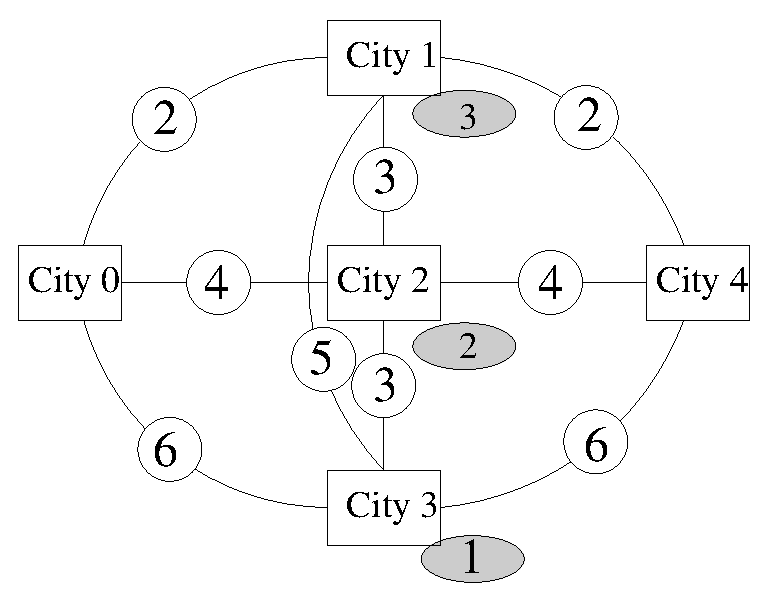
\includegraphics[width=0.5\textwidth]{./miniMulti.eps}
 % instance.eps: 0x0 pixel, 300dpi, 0.00x0.00 cm, bb=0 0 509 388
\caption{A schematic view of \MULTIZENO, a simple benchmark transportation problem: Durations of available flights are attached to the corresponding edges, costs/risks are attached to landing in the central cities (in the grey circles).}
\label{fig.instance}
\end{center}
\end{figure}

This section will detail the simple domain for multi-objective temporal planning that is described in Figure \ref{fig.instance}. The reader will have by now solved the little puzzle set in the Introduction, and found the solution with makespan 8 (flying 2 passengers to {\tt city 1}, one plane continues with its passenger to {\tt city 4} while the other plane flies back empty to {\tt city 0}, the plane in city {\tt city 4} returns empty to {\tt city 1} while the other plane brings the last passenger there, and the goal is reached after both planes bring both remaining passengers to {\tt city 4}). 

In order to turn this problem into a not-too-unrealistic logistics multi-objective problem, some costs, or risks, are added to all 3 central cities (1 to 3). This leads to two types of problems: In the \MULTIZENO$_{Cost}$, the second objective is an additive objective: each plane has to pay the corresponding tax every time it lands in that city; In the \MULTIZENO$_{Risk}$, the second objective is similar to a risk, and the maximal value encountered during the complete execution of a plan is to be minimized. 

In both cases however, there are 3 obvious points that belong to the Pareto Front: the solution with minimal makespan described above, and the similar solutions that use respectively {\tt city 2} and {\tt city 3} in lieu of {\tt city 1}. The values of the makespans are respectively 8, 16 and 24, and the values of the costs are, for each solution, 4 times the value of the single landing tax, and exactly the value of the involved risk. For the risk case, there is no other point on the Pareto Front, as a single landing on a high-risk city sets the risk of the whole plan to a high risk. For the cost model however, there are other points on the Pareto Front, as different cities can be used for the different passengers. For instance, in the case of Figure \ref{fig.instance}, this leads to a Pareto Front made of 5 points, (8,12), (16,8), and (24,4) (going only through {\tt city 1}, {\tt 2} and {\tt 3} respectively), plus (12,10) and (20,6), while only the first 3 are the Pareto Front in the risk case.

There are several ways to complexify this benchmark. A first possibility is to modify the relative values of the taxes/risks on the central cities: two sets of values will be used in the following, the (3-2-1) case depicted on Figure \ref{fig.instance}, and the (100-10-1) case (the one introduced in \cite{Schoenauer2006}), somehow representing another extreme of the spectrum of possible values. A second way is to add passengers. Sticking to bunches of 3 passengers in order to be able to easily derive some obvious Pareto-optimal solutions, 6 and 9 passengers will be experimented with, in addition to the simple case of 3 passengers. Finally, the number of central cities can be increased -- this will be the subject of on-going work.


\section{Experimental Results}
\label{sec:experiments}
This section presents an experimental analysis of the proposed approaches (Section \ref{sec:dae}) applied to the benchmark problems described above (Section \ref{benchmark}). 
The proposed approaches has been implemented within the \PARADISEO\ framework \url{http://paradiseo.gforge.inria.fr/}.

The default values for \DAEYAHSP\ internal parameters are taken from the reference paper~\cite{Bibai2010} and have not been further tuned for this work.
The population size for all MOEA variants has been set to $100$ individuals, and $1000$ generations were systematically run. Of course, all these parameters should be tuned in further work.
Furthermore, the embedded planner YAHSP  is constrained with a maximal number of expanded nodes. Depending on the complexity of the planning task, this number varies
from few  to thousands nodes. In our work this parameter takes values in the range $10 000$ to $1$ million and is determined during the initialization (see \cite{Bibai2010} for details).
%However, since our instances are relatively small, we have fixed this number to  $10^6$ .
% \begin{table*}[h]
% \centering
% \scriptsize
% \begin{tabular}{l c c c}
% \hline\hline
% Name & Min & Max & Default \\ 
% \hline
% Probability of crossover & 0.0 & 1 & 0.8 \\
% Probability of mutation & 0.0& 1& 0.2 \\
% Rate of mutation add station& 0& 10& 1 \\
% Rate of mutation delete station& 0& 10& 3 \\
% Rate of mutation add atom& 0& 10& 1 \\
% Rate of mutation delete atom& 0& 10& 1 \\
% Mean average for mutations& 0.0& 1& 0.8 \\
% %Time interval radius& 0& 10& 2 \\
% %Maximum number of stations& 5& 50& 20 \\
% Maximum number of nodes & 100& 10e6& 10e4 \\
% %Population size& 10& 300& 100 \\
% %Number of offspring & 100& 2 000& 700 \\
% \hline
% \end{tabular}
% \caption{Algorithm parameters}
% \label{table:parameters}
% \end{table*} 

\subsection{My Results}
\begin{itemize}
%Pareto Front found 
 \item 2 times by SPEA2 for the COST case 1-10-100
 \item 1 time by SPEA2 for the RISK case 1-10-100
%\item 
\end{itemize}


\subsection{Results}
To illustrate the search capabilities of our hybrid algorithms, we include in Figure~\ref{fig2:zenoParetofront} the Pareto fronts reached by the different algorithms
when solving the instance problem MultiZenoTravel with the second objective as the  total cost.
%For this instance, we compute by hand the optimal Pareto front that is constituted by five solutions when considering  the cost as second objective
In the case of MultiZenoTravel3$_{cost}$, we observe that the fronts obtained by  NSGA-II, IBEA$_{\epsilon^+}$ and SPEA2 have a better convergence and distribution of solutions than IBEA$_{H^-}$. 
Besides, all the solutions have converged towards the true Pareto front, while in IBEA$_{H^-}$ fronts some 
solutions have not. For the instance MultiZenoTravel6$_{cost}$ and  MultiZenoTravel9$_{cost}$, the fronts are quite similar between them, although we can appreciate some slight differences.\\
The evolution of the quality of solutions is computed according to $I_{H^-}$ indicator and is depicted for each instance in Figure~\ref{fig3:zenoHypervolume}.
In detail, the curves of Figure~\ref{fig3:zenoHypervolume} are  obtained on the  MultiZenoTravel instances by considering the second objective as total cost or risk.
At first sight, the outcomes obtained show that algorithms converge far more quickly towards the optimal Pareto front  when considering the
 risk case than  in the total cost case.
In detail, we can see that a great part of the optimization is achieved around the first 400  and 50 generations respectively for the cost and risk case and that the improvement of the quality of solutions is quite slow after these generations.
Depending on the instance, we can see two different scenarios:
When dealing with the total cost case (Figure~\ref{fig3:zenoHypervolume}(a,c, e)), it seems that for the instance MultiZenoTravel3$_{cost}$ and MultiZenoTravel9$_{cost}$ ,  NSGA-II outperforms SPEA2, IBEA$_{\epsilon^+}$ and IBEA$_{H^-}$.
While, on the instance MultiZenoTravel6$_{cost}$, it appears that the algorithms  are quite equivalent.\\
%If we are now interested in the realistic instances (Fig. 10(c, d)), the quality of solutions follows practically the
However, when considering the risk case (Figure~\ref{fig3:zenoHypervolume}(b,d, f)), the quality of solutions  for all algorithms 
follows practically the same evolution on the instances  MultiZenoTravel3$_{risk}$ and  MultiZenoTravel6$_{risk}$. 
Even if the  convergence of SPEA appears to be a bit slower than the other algorithms.
Whilst on MultiZenoTravel9$_{risk}$, the other algorithms are better in terms of convergence than SPEA2.
It is interesting to note that the size of instances  and the  second considered objective, seem to  influence the efficiency of the algorithms.
SPEA2 and IBEA$_{\epsilon^+}$  provide  better solutions on small instances,  whereas NSGA-II and IBEA$_{H^-}$ have better convergence and distribution  towards the optimal Pareto front on 
large instances. However, the performances are similar when considering the risk as second objective except for MultiZenoTravel9$_{risk}$.
%Depending on the instance, we can see that two different scenarios:
\subsection{Performance Assessment}
 A set of 30 runs per instance has been performed for each algorithms.
% In order to evaluate the quality of the approximations for every
%instance, we follow the protocol proposed in~\cite{Fonseca2005}.
% For a given instance, let $Z^{all}$ denote the union of the outputs that
% we obtained during all our experiments. Note that this set probably contains both dominated and non-dominated points, as a given approximation may contain
% vectors dominating the ones of another approximation, and vice versa.\\
% We first compute a reference set $Z^*_N$ containing all the non-dominated points of $Z^{all}$. 
% Second, we define $z^{min} = (z^{min}_1 ,\ldots, z^{min}_n)$ an $z^max =(z^{max}_1 ,\ldots, z^{max}_n)$, where $z^{min}_k$ (resp. $z^{max}_k$) denotes the lower (resp. upper)
%  bound for the $k^{th}$ objective for all the points contained in $Z^{all}$.
% In order to give a roughly equal range to the objective functions, values are normalized with respect to $z^min$ and $z^{max}$.
% Then, to measure the quality of an output set $A$ in comparison to $Z^*_N$ , we compute the difference between these two sets by using the unary hypervolume
% metric~\cite{Zitzler2004}, $z^{max}$ being the reference point. 
In order to measure the quality of an output set of solutions $A$ in comparison to a reference set $Z^*_N$, we compute the difference between these two sets by using the unary hypervolume
metric~\cite{Zitzler2004}. The hypervolume computes the volume (in objective function space) comparatively to $Z^*_N$. The closer this measure to 0, the better is the approximation $A$.
%. The hypervolume difference indicator ($I^-_H $) computes the portion of the objective
%space that is weakly dominated by $Z^*_N$ and not by $A$. The closer this measure to 0, the better is the approximation $A$~\cite{Zitzler2004}.
% Furthermore, we also consider the additive $\epsilon$-indicator proposed in~\cite{Zitzler2004}. %The unary additive $\epsilon$-indicator ($I^1_{\epsilon^+}$ ) gives the minimum factor by which an approximation $A$ has to be translated in the objective
%space to dominate the reference set $Z^*_N$. 
%Note that both $I^-_H $  and $I^1_{\epsilon^+}$ values are to be minimized. and $I^1_{\epsilon^+}$  measures
Thus, for each test instance, we obtain 30 $I^-_H $ measures  corresponding to the 30  runs performed for each algorithm. 
Once all these values are computed, we perform a statistical analysis for a pairwise comparison of methods. To this end, we use the Wilcoxon signed rank test. For a given
test instance, and with respect to a \textit{p}-value of 0.05 and to the metric under consideration, this statistical test reveals if
the sample of approximation sets obtained by a given search method is significantly better than the one of another search
method, or if there is no significant difference between both of them. Note that all the performance assessment procedures have been achieved using
the performance assessment tool suite provided in PISA\footnote{http://www.tik.ee.ethz.ch/pisa/}.%~\cite{Bleuler2003}.

A widely-used way to compare different multi-objective algorithms is to perform statistical tests based on the evolution of some measure of performance during several runs. The $I^-_H $ metric has been chosen here, using as reference set the union of all solutions found by at least one run of one algorithm.
Wilcoxon signed rank tests with confidence level 0.05 using this $I^-_H $ metric have been done on the results for all instances (zeno3-6-9) and all variants of \MODAE\ (NSGA-II, SPEA2, IBEA$_{Hyp}$ and IBEA$_{Eps}$: Except for the MultiZenoTravel6$_{risk}$ instance, where  SPEA2 appears to be less efficient that all other algorithms, 
no statistical difference appears. 
\begin{figure*}[h]
 \centering{
 \subfloat[MultiZenoTravel3$_{cost}$]{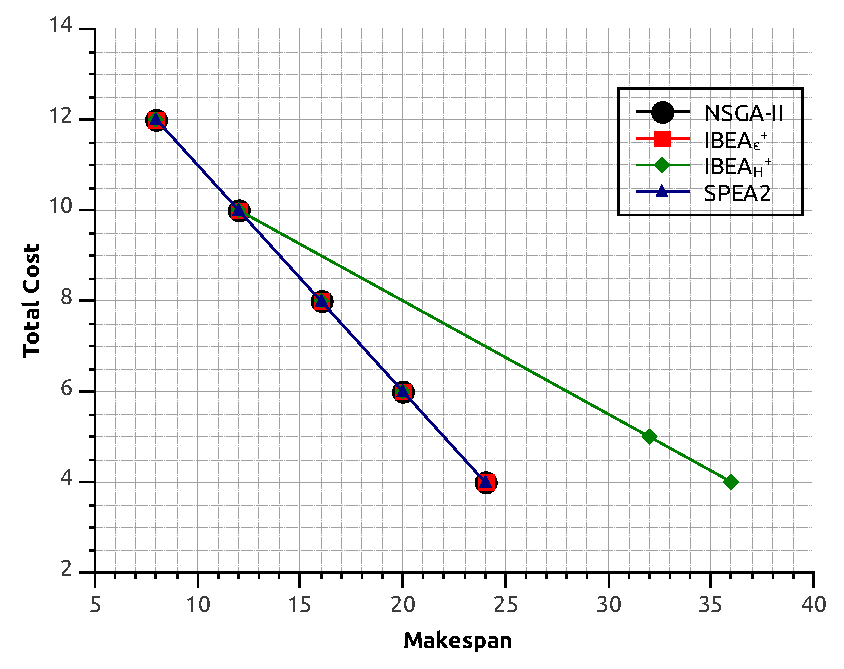
\includegraphics[bb=0 0 389 305, scale=0.35]{./paretofrontZeno3ewAdd.eps}
\label{fig2-a:zeno3AddParetofrontareto}}
\subfloat[MultiZenoTravel6$_{cost}$]{ 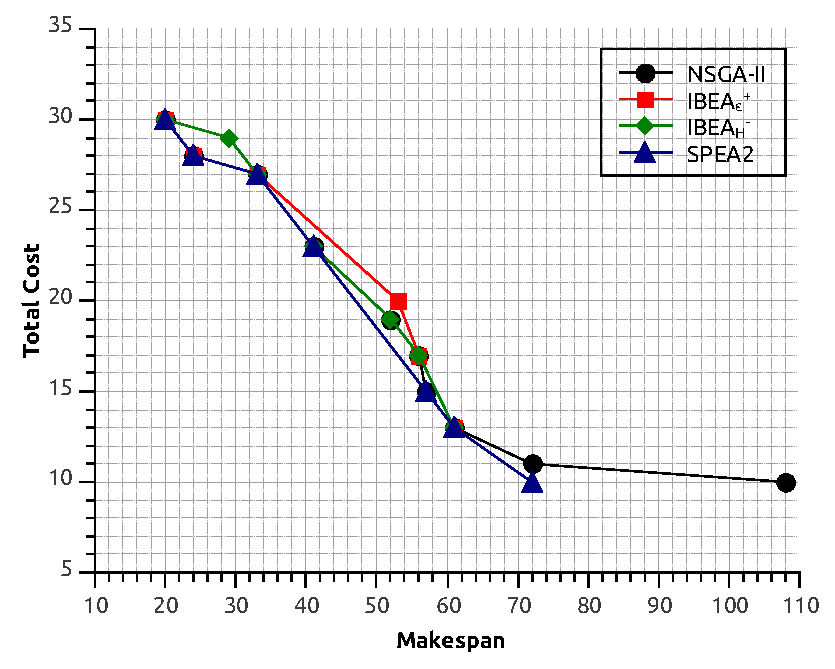
\includegraphics[bb=0 0 385 305, scale=0.35]{./paretofrontZeno6ewAdd.eps}
\label{fig2-b:zeno6AddParetofrontareto}}\\
 % nsgaZenoMax.eps: 0x0 pixel, 300dpi, 0.00x0.00 cm, bb=0 0 374 278 
 \subfloat[MultiZenoTravel9$_{cost}$]{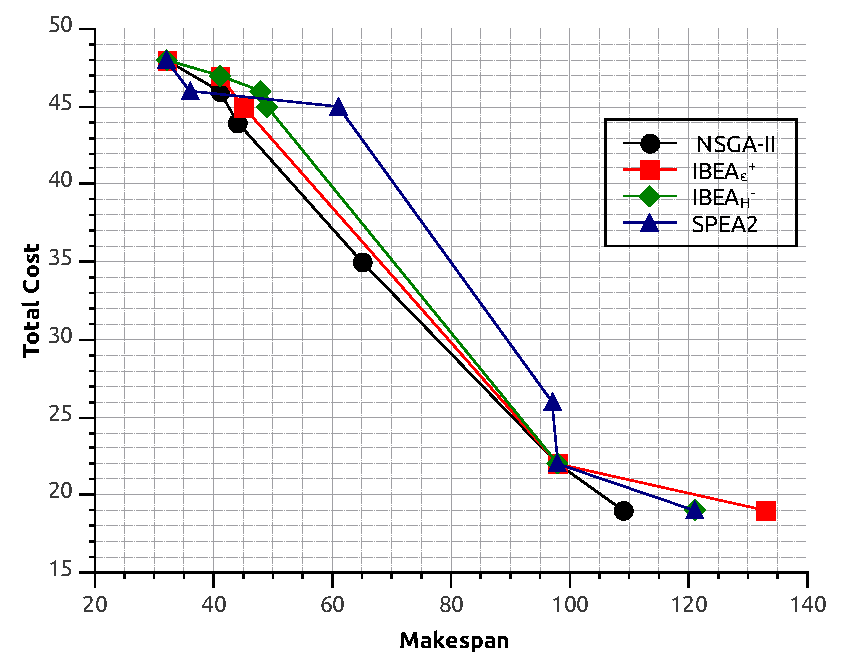
\includegraphics[bb=0 0 389 305, scale=0.35]{./paretofrontZeno9ewAdd.eps}
\label{fig2-c:zeno9AddParetofrontareto}}
 % paretofrontZeno9ewAdd.eps: 0x0 pixel, 300dpi, 0.00x0.00 cm, bb=0 0 389 305
 \caption{Pareto fronts of the \MULTIZENO\ instances.}
 \label{fig2:zenoParetofront}}
\end{figure*}


\begin{figure*}[h]
 \centering{
\subfloat[MultiZenoTravel3$_{cost}$]{ 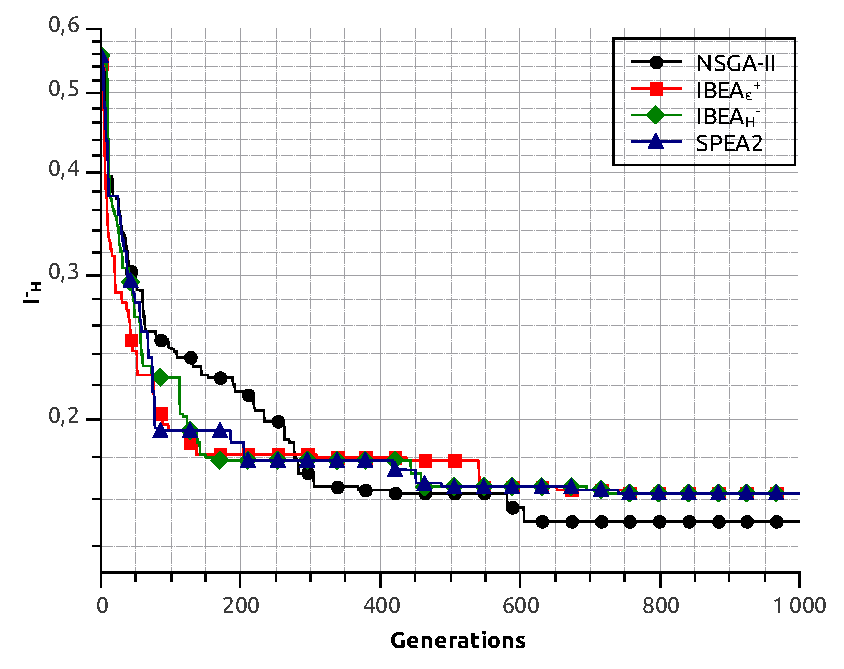
\includegraphics[bb=0 0 389 305, scale=0.35]{./hypervolumeZeno3ewAddmedian.eps}
 % hypervolumeZeno3Addmedian.eps: 0x0 pixel, 300dpi, 0.00x0.00 cm, bb=0 0 389 305
\label{fig3-a:zeno3Hypervolume}}
 \subfloat[MultiZenoTravel3$_{risk}$]{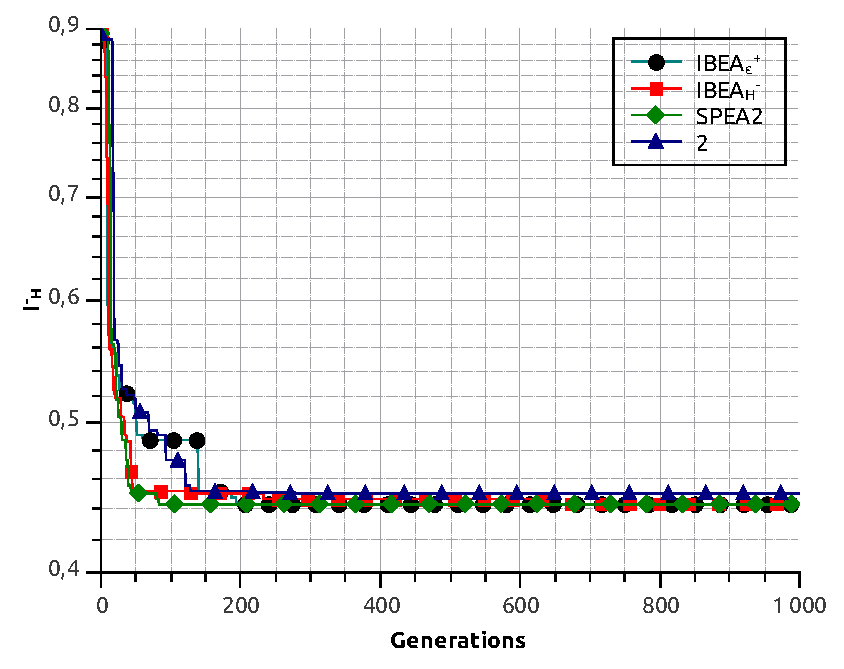
\includegraphics[bb=0 0 389 305, scale=0.35]{./hypervolumeZeno3ewMaxmedian.eps}
 % hypervolumeZeno3Maxmedian.eps: 0x0 pixel, 300dpi, 0.00x0.00 cm, bb=0 0 378 308
\label{fig3-a:zeno3Hypervolume}} \\
 \subfloat[MultiZenoTravel6$_{cost}$]{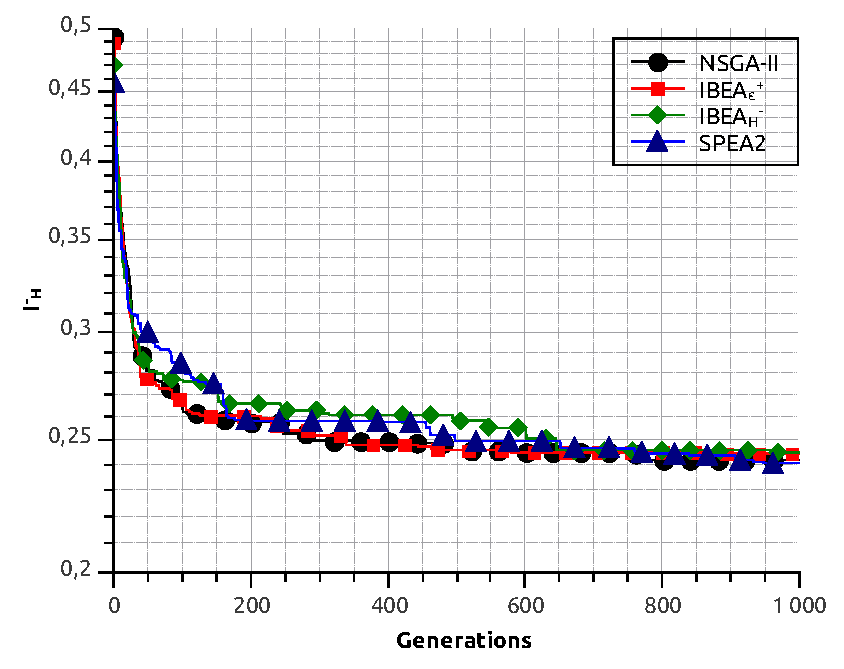
\includegraphics[bb=0 0 389 305, scale=0.35]{./hypervolumeZeno6ewAddmedian.eps}
%  % hypervolumeZeno6Addmedian.eps: 0x0 pixel, 300dpi, 0.00x0.00 cm, bb=0 0 389 305
\label{fig3-a:zeno6Hypervolume}}  
\subfloat[MultiZenoTravel6$_{risk}$]{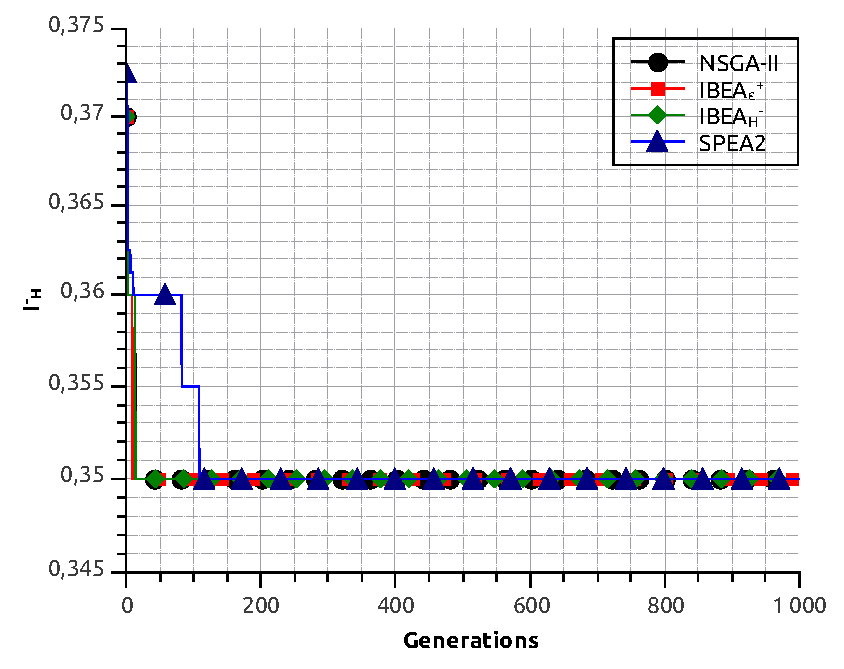
\includegraphics[bb=0 0 389 305, scale=0.35]{./hypervolumeZeno6ewMaxmedian.eps}
%  % hypervolumeZeno6Maxmedian.eps: 0x0 pixel, 300dpi, 0.00x0.00 cm, bb=0 0 389 305
\label{fig3-a:zeno6Hypervolume}}  \\
\subfloat[MultiZenoTravel9$_{cost}$]{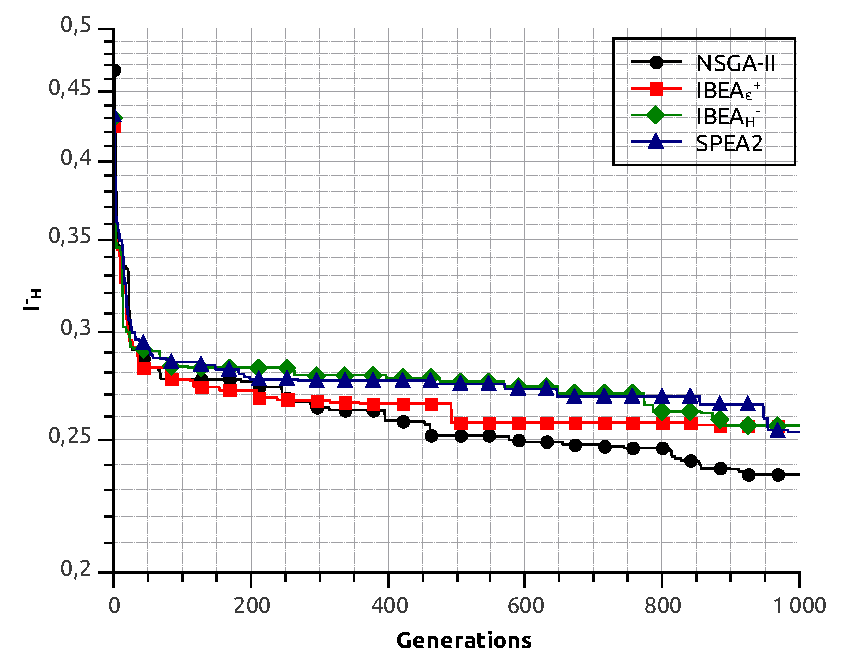
\includegraphics[bb=0 0 389 305, scale=0.35]{./hypervolumeZeno9ewAddmedian.eps}
%  % hypervolumeZeno6Addmedian.eps: 0x0 pixel, 300dpi, 0.00x0.00 cm, bb=0 0 389 305
\label{fig3-a:zeno9Hypervolume}}  
\subfloat[MultiZenoTravel9$_{risk}$]{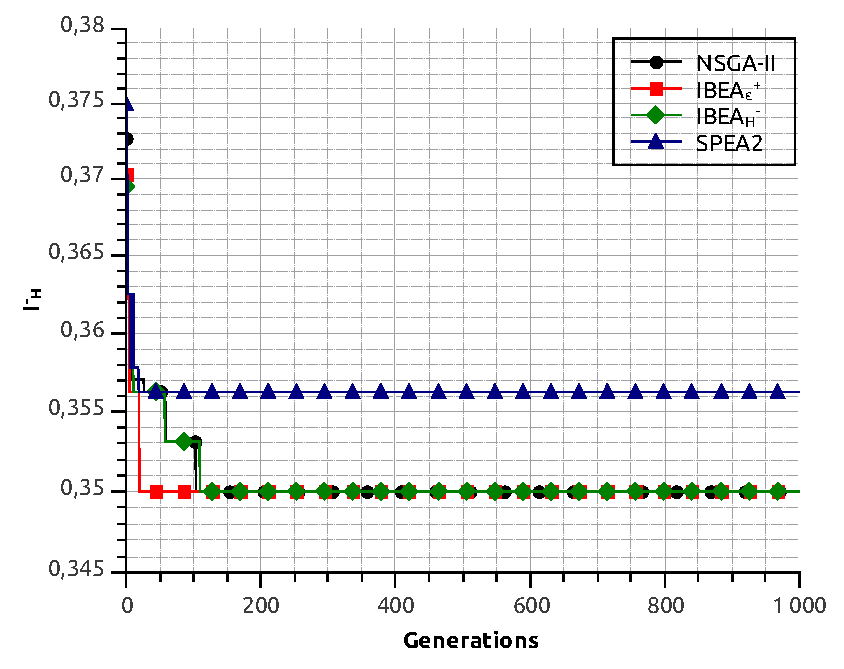
\includegraphics[bb=0 0 389 305, scale=0.35]{./hypervolumeZeno9ewMaxmedian.eps}
\label{fig3-a:zeno9Hypervolume}}
\caption{Median evolution of the quality of solutions on \MULTIZENO\ instances  according to Hypervolume indicator $I_{H^-}$ over 30 runs.}

 \label{fig3:zenoHypervolume}}
\end{figure*}


\section{Discussion}
\label{sec:discussion}
The multi-objectivization of \DAEX\ was sketched in \cite{Schoenauer2006}. However, the primitive version of \DAEX\ that it relied on was rather limited, and required a lot of human expertise in order to choose which predicate to use in the representation of states.

Though the Pareto dominance, and hence the Pareto-based ranking and strength computations, are comparison-based, the indicators are not -- hence the differences observed between the 3-2-1 and the 100-10-1 costs for cities 1-3. 

Parameter tuning



\section{Conclusion \& Perspectives}
\label{sec:conclusion}
Building on the very preliminary work in \cite{Schoenauer2006}, the contributions of this paper are twofold. Firstly, \MULTIZENO, an original benchmark domain for multi-objective temporal planning has been detailed, and several levers identified that allow to generate more or less complex instances: increasing the number of passengers obviously makes the problem more difficult; modifying the costs of the cities and the durations of the flights is another path for complexification, though deeper work is required to identify the consequences of each modification.
Secondly, several multi-objectivization of \DAEX, an efficient evolutionary planner in the single-objective case, have been proposed, based on 4 popular MOEAs (NSGA-II, SPEA2, and two variants of IBEA).
However, the experimental comparisons of those variants on the discrete \MULTIZENO\ benchmark raises more questions than it brings answers: the sparseness of the Pareto Front for the small instances has been identified as a possible source for the rather poor performances of all variants, and suggests that rather different strategies should be designed in such contexts. Another direction of research, more directly linked to the proposed \MODAE\ approach,  is of course to combat the non-symmetry of the results, due to the fact that the embedded planner is single objective, and at the moment only optimizes on one objective, letting evolution handle the trade-offs. A straightforward modification is to alternate some way or another the optimization by the embedded planner between both objectives, or more generally to use some aggregation of the objective within the embedded planner: this is the subject of on-going work. 

\bibliographystyle{splncs}
\bibliography{ppsnb}


\end{document}


Mail de Vincent
===============

2 papiers d'avant PDDL3.0 :

@article{do2003sapa,
  title={Sapa: A multi-objective metric temporal planner},
  author={Do, M.B. and Kambhampati, S.},
  journal={J. Artif. Intell. Res. (JAIR)},
  volume={20},
  pages={155--194},
  year={2003}
}

@article{refanidis2003multiobjective,
  title={Multiobjective heuristic state-space planning},
  author={Refanidis, I. and Vlahavas, I.},
  journal={Artificial Intelligence},
  volume={145},
  number={1},
  pages={1--32},
  year={2003},
  publisher={Elsevier}
}


Depuis PDDL3.0, dont la ref est dessous, tous les planners du track
"net-benefit" sont censés résoudre ce type de problème (multi-objectifs avec
aggrégation) :

@inproceedings{gerevini2006preferences,
  title={Preferences and soft constraints in PDDL3},
  author={Gerevini, A. and Long, D.},
  booktitle={ICAPS Workshop on Planning with Preferences and Soft Constraints},
  pages={46--53},
  year={2006}
}



Gagnant 2006 : SGPLAN

@article{chen2006temporal,
  title={Temporal planning using subgoal partitioning and resolution in SGPlan},
  author={Chen, Y. and Wah, B.W. and Hsu, C.W.},
  journal={Journal of Artificial Intelligence Research},
  volume={26},
  number={1},
  pages={323--369},
  year={2006},
  publisher={AI Access Foundation}
}

Gagnant 2008 : GAMER

@inproceedings{edelkamp2009optimal,
  title={Optimal symbolic planning with action costs and preferences},
  author={Edelkamp, S. and Kissmann, P.},
  booktitle={Proc. of the 21st International Joint Conference on Artificial Intelligence (IJCAI 2009)},
  pages={1690--1695},
  year={2009}
}

Compétition 2011 : track net-benefit annulée !
